%% 
%% Copyright 2007, 2008, 2009 Elsevier Ltd
%% 
%% This file is part of the 'Elsarticle Bundle'.
%% ---------------------------------------------
%% 
%% It may be distributed under the conditions of the LaTeX Project Public
%% License, either version 1.2 of this license or (at your option) any
%% later version.  The latest version of this license is in
%%    http://www.latex-project.org/lppl.txt
%% and version 1.2 or later is part of all distributions of LaTeX
%% version 1999/12/01 or later.
%% 
%% The list of all files belonging to the 'Elsarticle Bundle' is
%% given in the file `manifest.txt'.
%% 

%% Template article for Elsevier's document class `elsarticle'
%% with numbered style bibliographic references
%% SP 2008/03/01

\documentclass[preprint,12pt, a4paper]{elsarticle}

%% Use the option review to obtain double line spacing
%% \documentclass[authoryear,preprint,review,12pt]{elsarticle}

%% For including figures, graphicx.sty has been loaded in
%% elsarticle.cls. If you prefer to use the old commands
%% please give \usepackage{epsfig}

%% The amssymb package provides various useful mathematical symbols
\usepackage{amssymb}
%% The amsthm package provides extended theorem environments
%% \usepackage{amsthm}

%% The lineno packages adds line numbers. Start line numbering with
%% \begin{linenumbers}, end it with \end{linenumbers}. Or switch it on
%% for the whole article with \linenumbers.
\usepackage{lineno}

\usepackage{float}
\restylefloat{table}

\journal{SoftwareX}

\begin{document}

\begin{frontmatter}

%% Title, authors and addresses

%% use the tnoteref command within \title for footnotes;
%% use the tnotetext command for theassociated footnote;
%% use the fnref command within \author or \address for footnotes;
%% use the fntext command for theassociated footnote;
%% use the corref command within \author for corresponding author footnotes;
%% use the cortext command for theassociated footnote;
%% use the ead command for the email address,
%% and the form \ead[url] for the home page:
%% \title{Title\tnoteref{label1}}
%% \tnotetext[label1]{}
%% \author{Name\corref{cor1}\fnref{label2}}
%% \ead{email address}
%% \ead[url]{home page}
%% \fntext[label2]{}
%% \cortext[cor1]{}
%% \address{Address\fnref{label3}}
%% \fntext[label3]{}

\title{CNATool - Complex Network Analysis Tool}

%% use optional labels to link authors explicitly to addresses:
%% \author[label1,label2]{}
%% \address[label1]{}
%% \address[label2]{}

\author[cimatec]{Renata Souza Freitas Dantas Barreto}
\ead{renatasouzabarreto@gmail.com}
\author[cimatec]{Hernane Borges de Barros Pereira}
\ead{hernane@fieb.org.br}
\author[cimatec]{Roberto Luiz Souza Monteiro}
\ead[url]{http://www.souzamonteiro.com}
\ead{roberto.monteiro@fieb.org.br}
\address[cimatec]{SENAI CIMATEC University Center\\Av. Orlando Gomes, 1845,\\Piat\~{a},\\Salvador - BA,\\41650-010}

\begin{abstract}
%% Text of abstract 
CNATool is an online program for analyzing complex and social networks.
It was developed using the MaiaScript programming language to allow
quick and simplified analysis of graphs of complex networks
from any device connected to the Internet. Currently it supports load graphs
in Pajek and JSON formats, create artificial graphs (random, scale-free,
small word and hybrid), display network graph, layout graph,
graph properties (average degree, density, average clustering coefficient,
average shortest path, diameter and graph efficiency, display detailed properties of
vertices (degrees, clustering and centrality), save graph in Pajek format,
export graph in SVG format, save a summary of graph’s properties in HTML format.
\end{abstract}

\begin{keyword}
%% keywords here, in the form: keyword \sep keyword
graph \sep network \sep degree \sep clustering \sep centrality \sep Pajek

%% PACS codes here, in the form: \PACS code \sep code

%% MSC codes here, in the form: \MSC code \sep code
%% or \MSC[2008] code \sep code (2000 is the default)

\end{keyword}

\end{frontmatter}

\section*{Code metadata}
\label{metadata}

\begin{table}[H]
\begin{tabular}{|l|p{6.5cm}|p{6.5cm}|}
\hline
\textbf{Nr.} & \textbf{Code metadata description} & \textbf{Please fill in this column} \\
\hline
C1 & Current code version & 1.4.1 \\
\hline
C2 & Permanent link to code/repository used for this code version & $https://github.com/souzamonteiro/cnatool.git$ \\
\hline
C3 & Web site & $http://www.maiascript.com/maiascript/cnatool$ \\
\hline
C4 & Legal Code License & Apache-2.0 License \\
\hline
C5 & Code versioning system used & git \\
\hline
C6 & Software code languages, tools, and services used & MaiaScript, JavaScript, HTML \& CSS \\
\hline
C7 & Compilation requirements, operating environments & Node.js \\
\hline
C8 & If available Link to developer documentation/manual & $http://www.maiascript.com/cnatool/doc/cna/1.3.6/index.html$ \\
\hline
C9 & Support email for questions & $support@souzamonteiro.com$ \\
\hline
\end{tabular}
\caption{Code metadata}
\label{} 
\end{table}

\linenumbers

%% main text

\section{Motivation and significance}
\label{motivation}

\cite{Barabasi1999}
Introduce the scientific background and the motivation for developing the software.

Explain why the software is important, and describe the exact (scientific) problem(s) it solves.

Indicate in what way the software has contributed (or how it will contribute in the future) to the process of scientific discovery; if available, this is to be supported by citing a research paper using the software.

Provide a description of the experimental setting (how does the user use the software?).

Introduce related work in literature (cite or list algorithms used, other software etc.).


\section{Software description}
\label{description}

\begin{figure}[!htbp]
    \begin{center}
        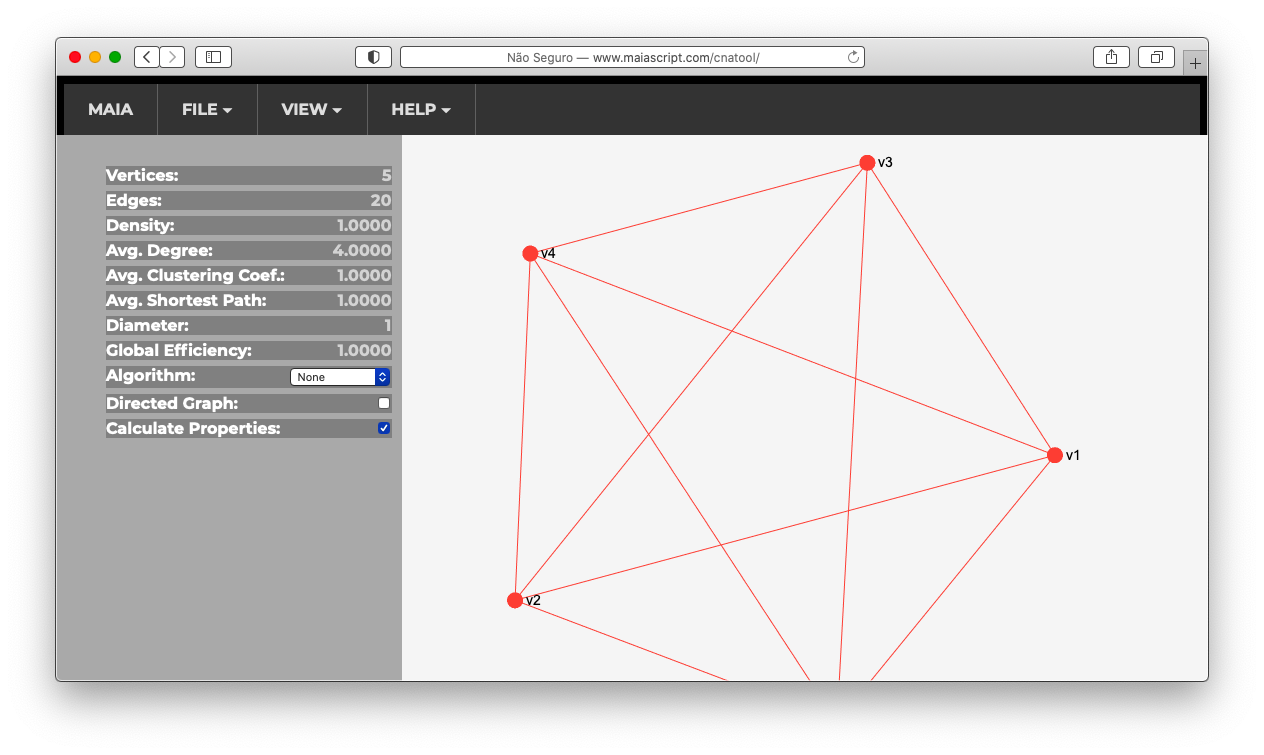
\includegraphics[scale=0.2]{images/macbook.png}
    \end{center}
    \caption{Screen of the CNATool program running on the Safari desktop browser. Source: Author..}
    \label{fig:macbook}
\end{figure}

\begin{figure}[!htbp]
    \begin{center}
        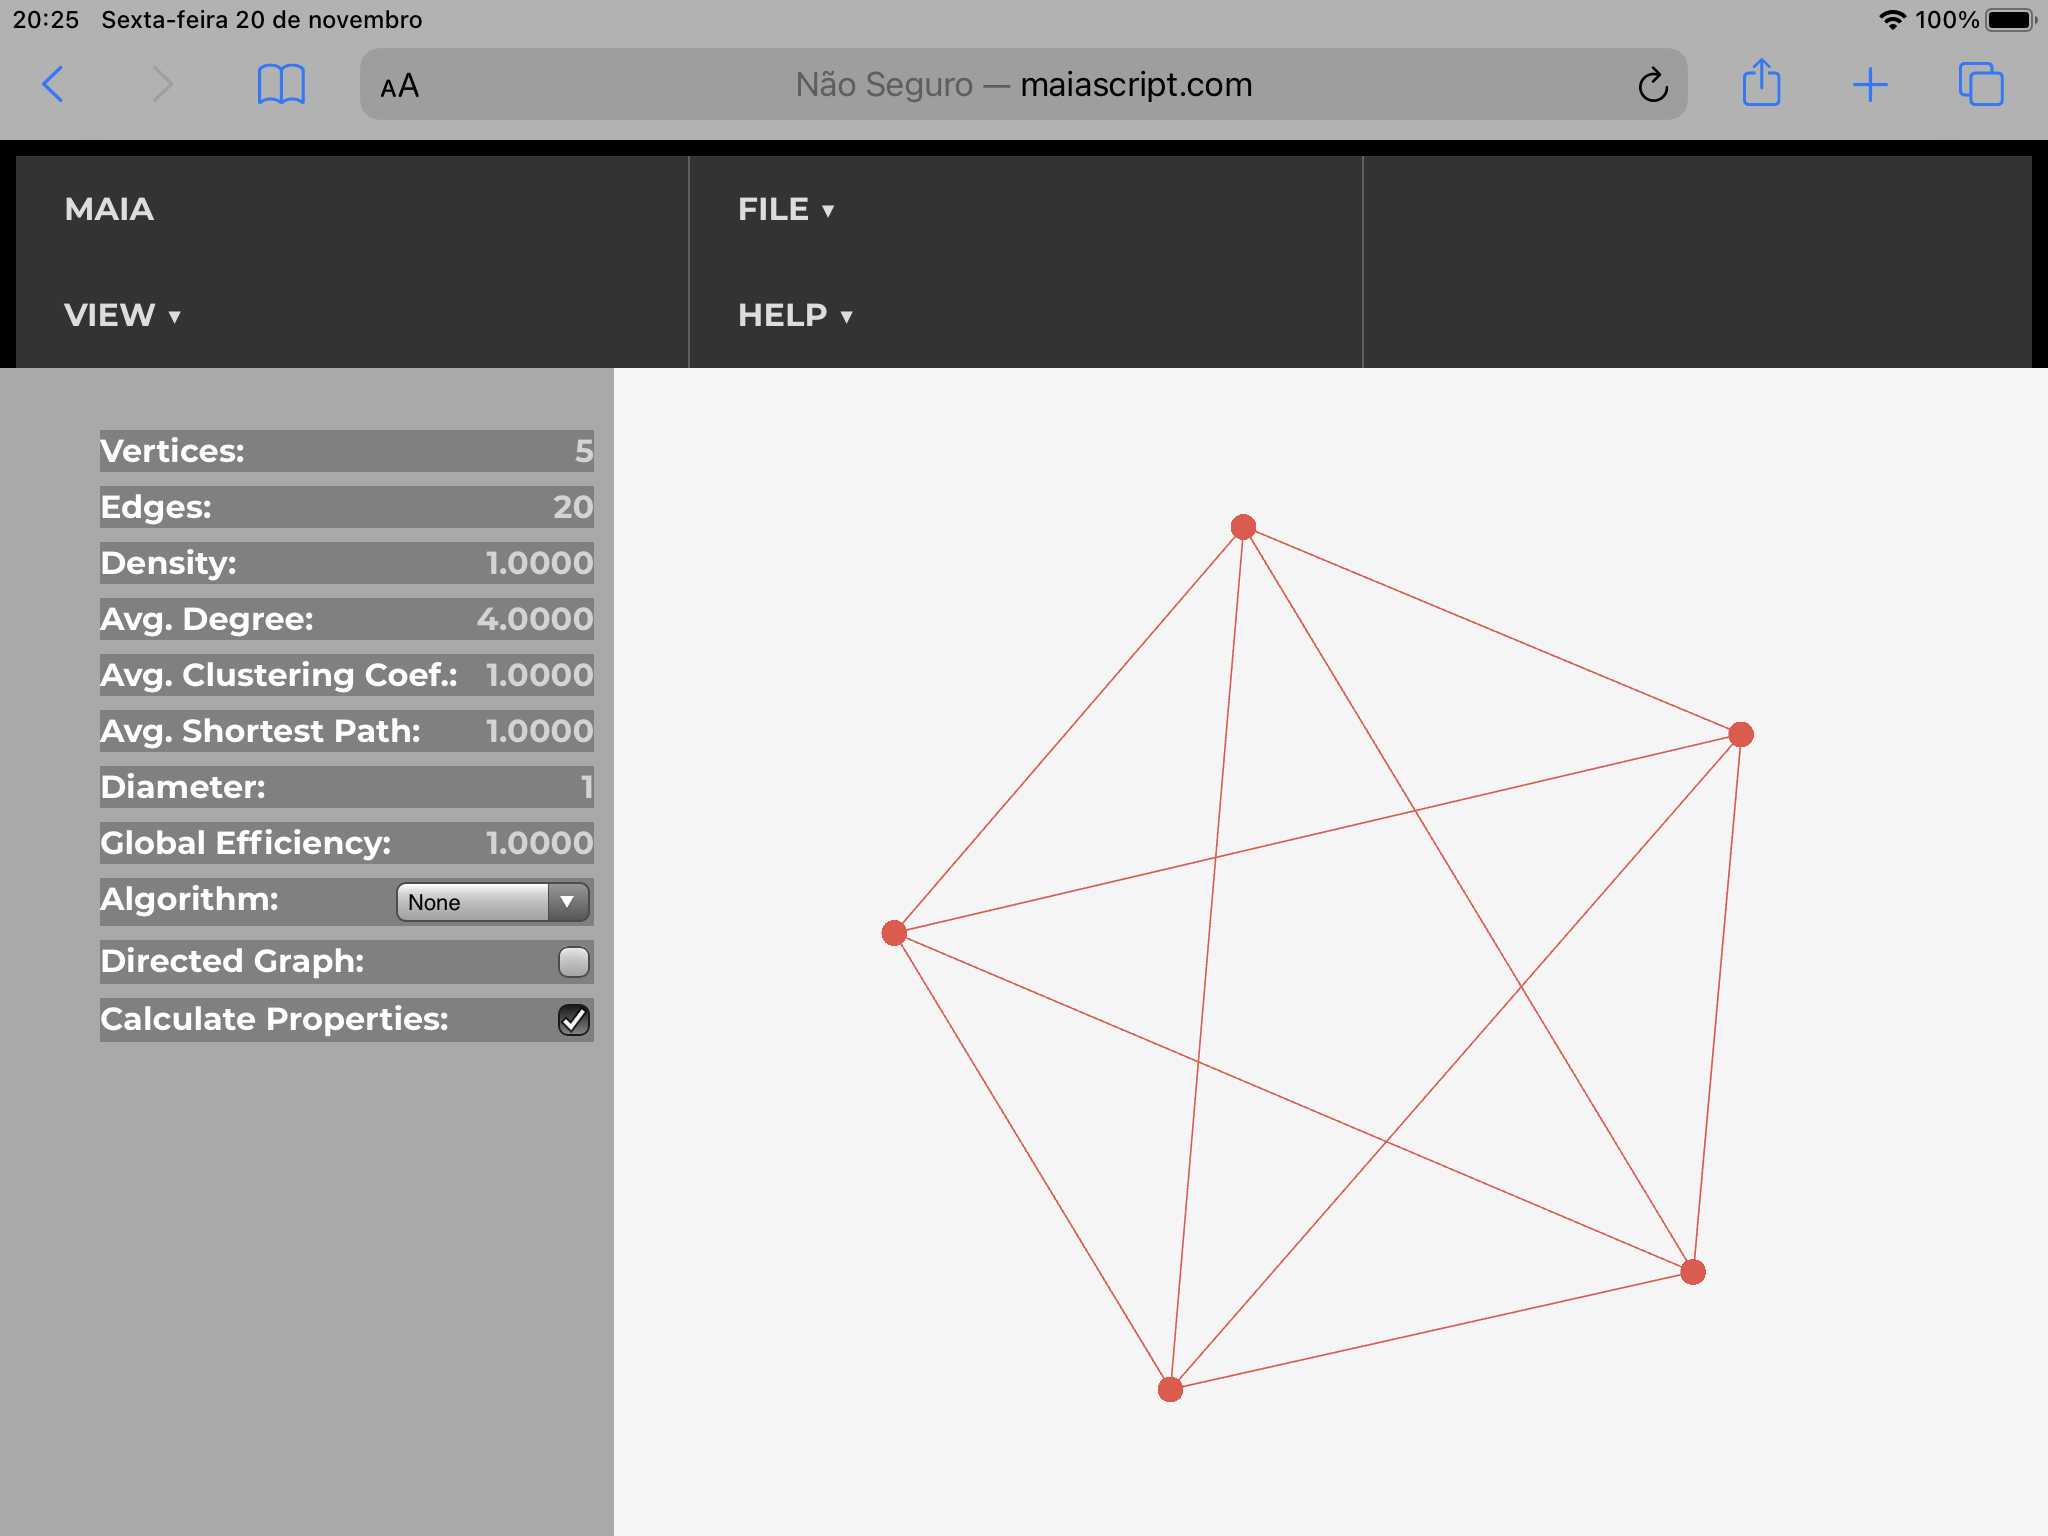
\includegraphics[scale=0.2]{images/ipad.png}
    \end{center}
    \caption{Screen of the CNATool program running on the Safari mobile browser on iPad. Source: Author.}
    \label{fig:ipad}
\end{figure}

\begin{figure}[!htbp]
    \begin{center}
        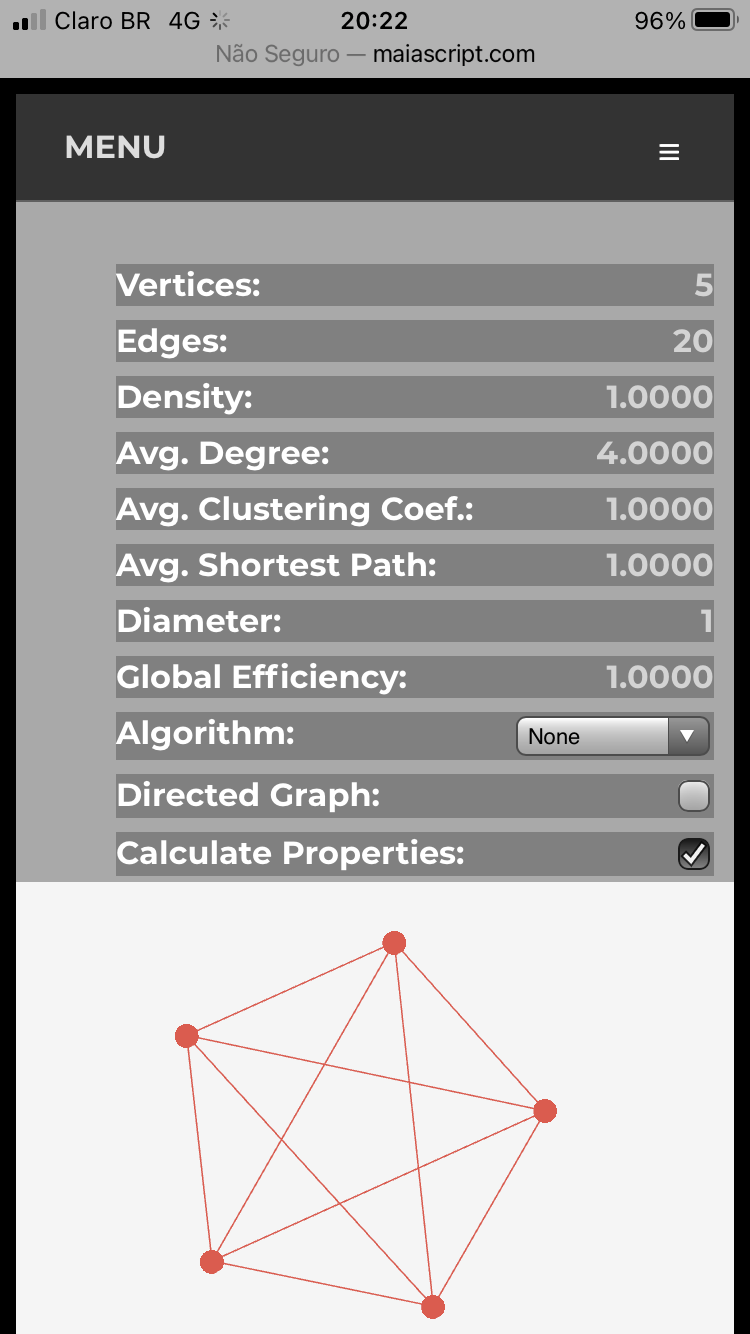
\includegraphics[scale=0.2]{images/iphone.png}
    \end{center}
    \caption{Screen of the CNATool program running on the Safari mobile browser on iPhone. Source: Author.}
    \label{fig:iphone}
\end{figure}

\subsection{Software Architecture}
\label{architecture}

\begin{figure}[!htbp]
    \begin{center}
        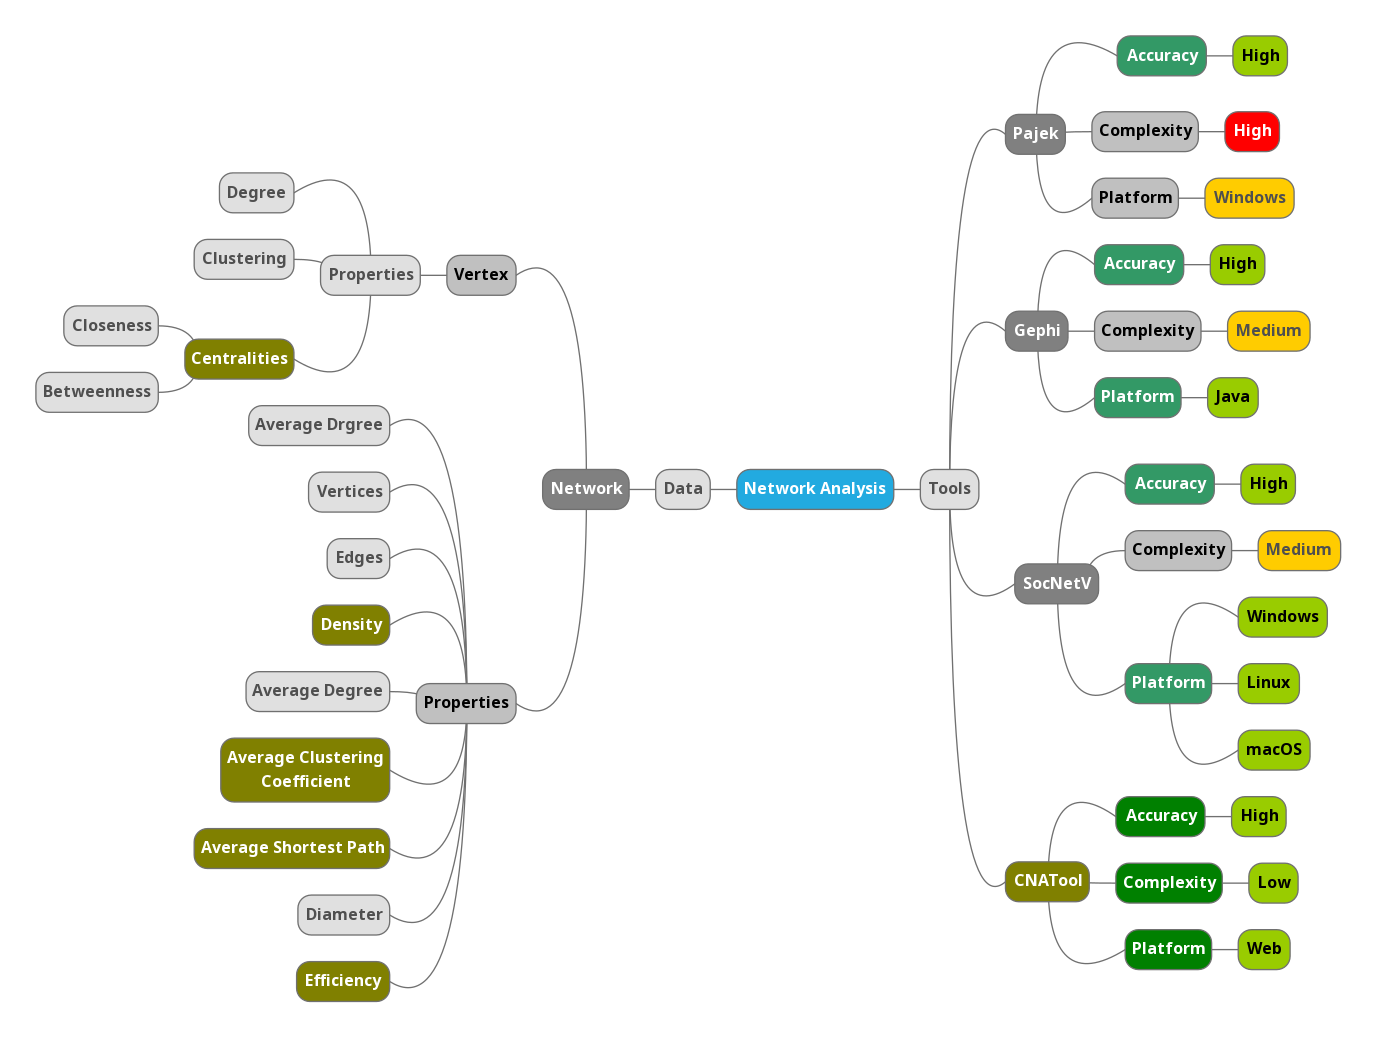
\includegraphics[scale=0.3]{images/mindmap.png}
    \end{center}
    \caption{Mind map of the main concepts involved in social and complex network analysis. Source: Author.}
    \label{fig:mindmap}
\end{figure}

\begin{figure}[!htbp]
    \begin{center}
        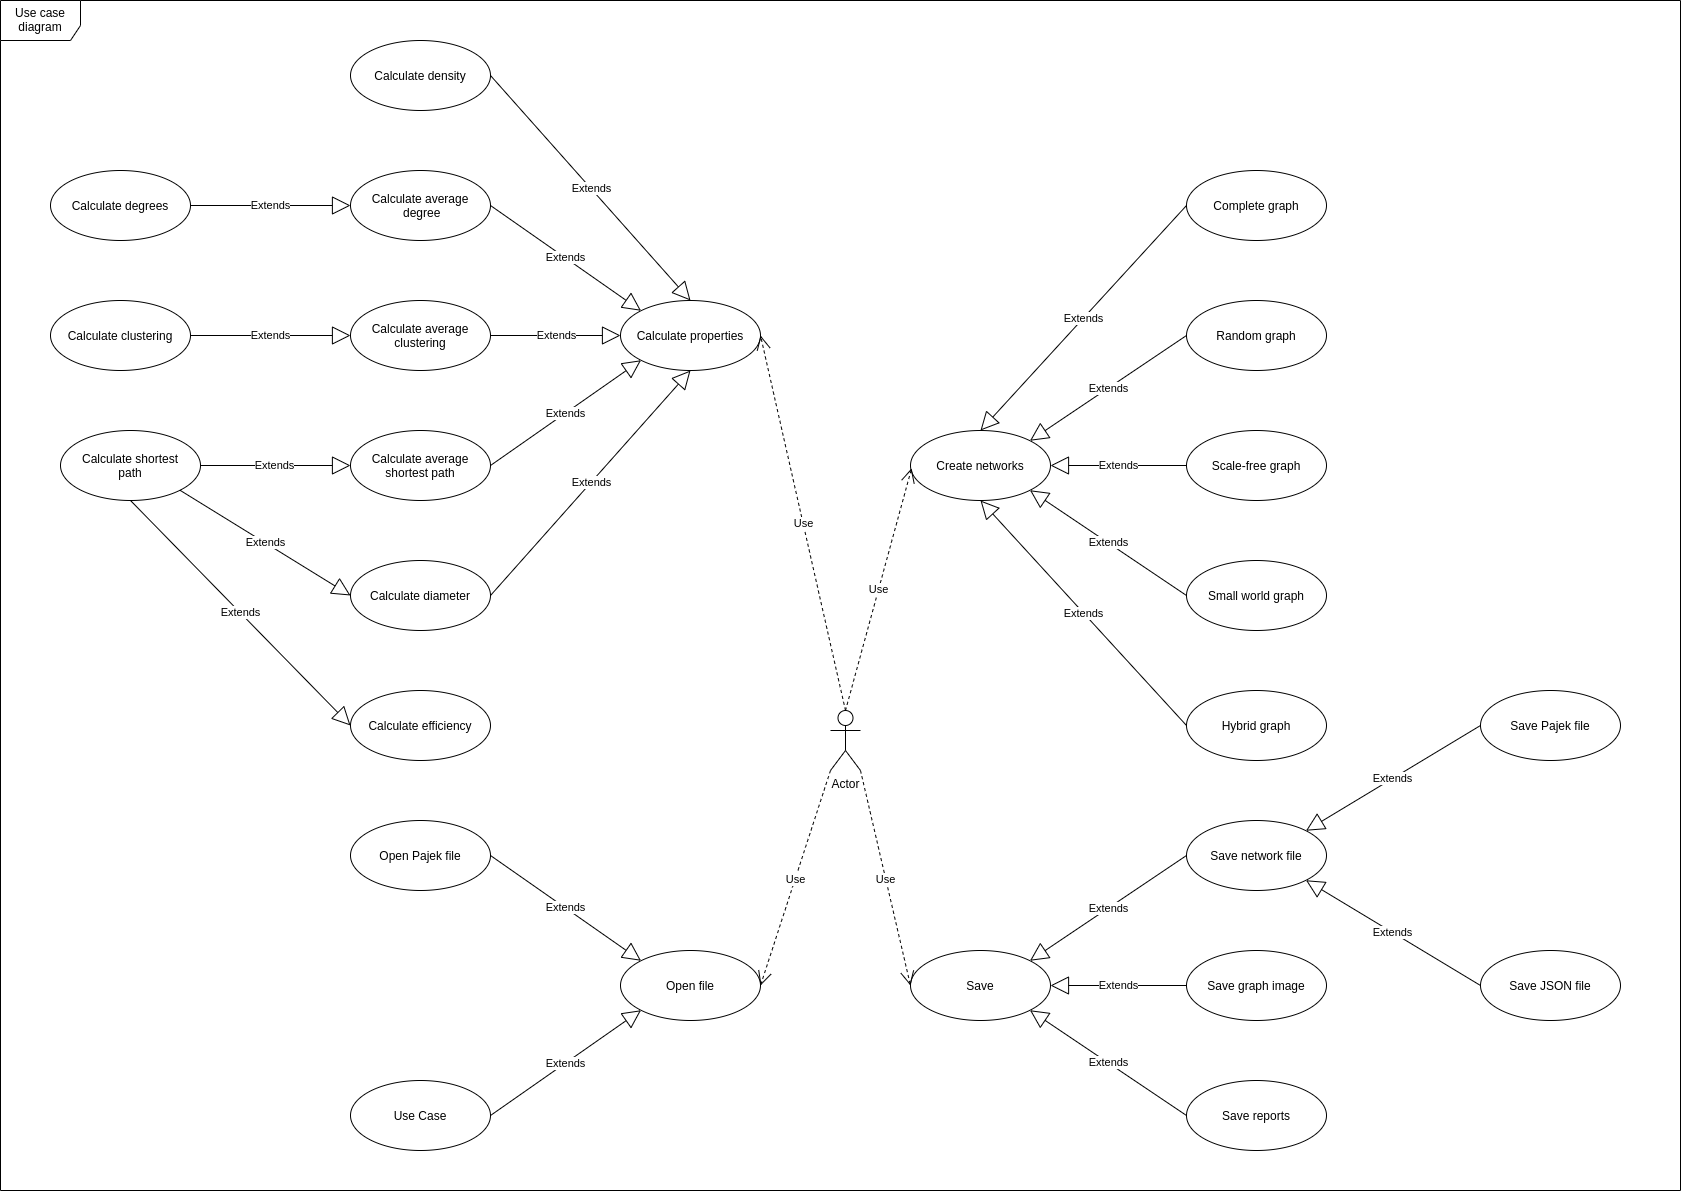
\includegraphics[scale=0.25]{images/use-case.png}
    \end{center}
    \caption{Use cases diagram for the CNATool program. Source: Author.}
    \label{fig:usecase}
\end{figure}

\begin{figure}[!htbp]
    \begin{center}
        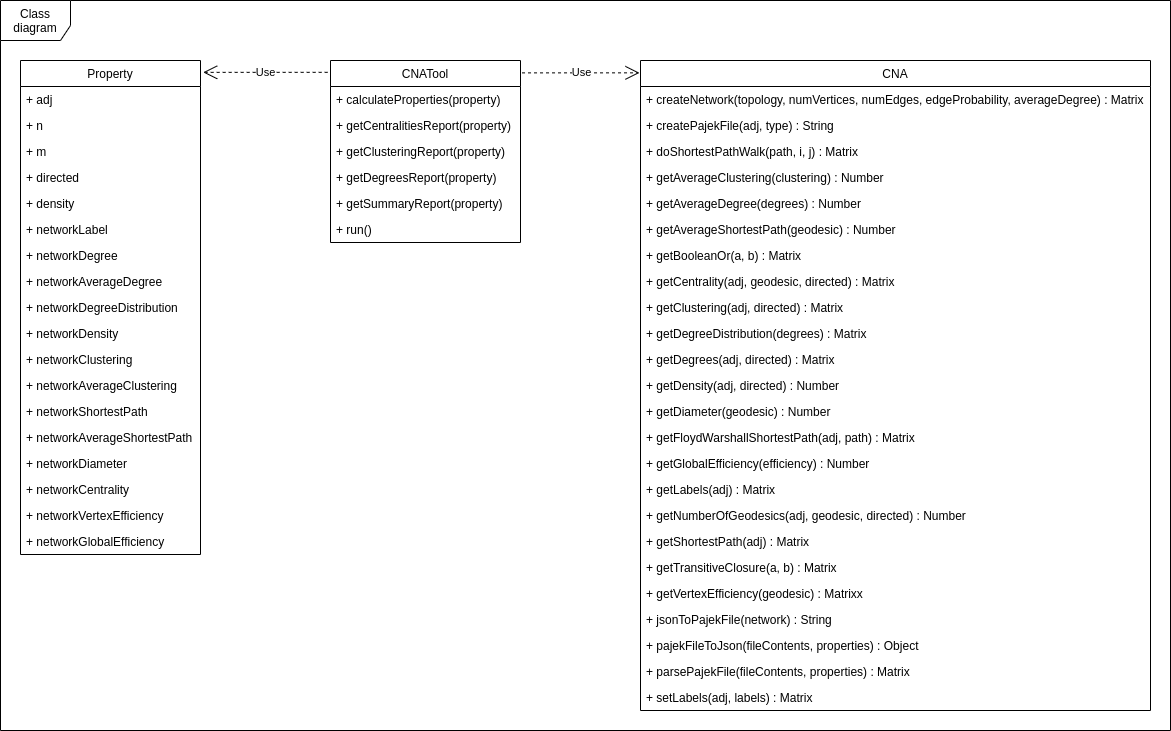
\includegraphics[scale=0.3]{images/class-diagram.png}
    \end{center}
    \caption{Class diagram for the CNATool program. Source: Author.}
    \label{fig:classdiagram}
\end{figure}

\begin{figure}[!htbp]
    \begin{center}
        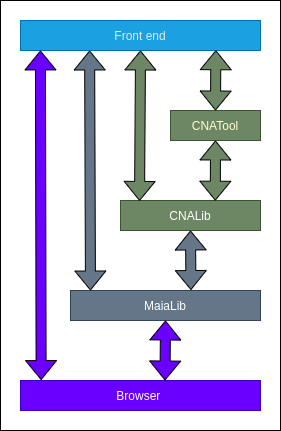
\includegraphics[scale=0.5]{images/architecture.png}
    \end{center}
    \caption{Architecture diagram for the CNATool program. Source: Author.}
    \label{fig:architecture}
\end{figure}

\subsection{Software Functionalities}
\label{functionalities}

Present the major functionalities of the software.

\subsection{Sample code snippets analysis}
\label{code}

\begin{figure}[!htbp]
    \begin{center}
        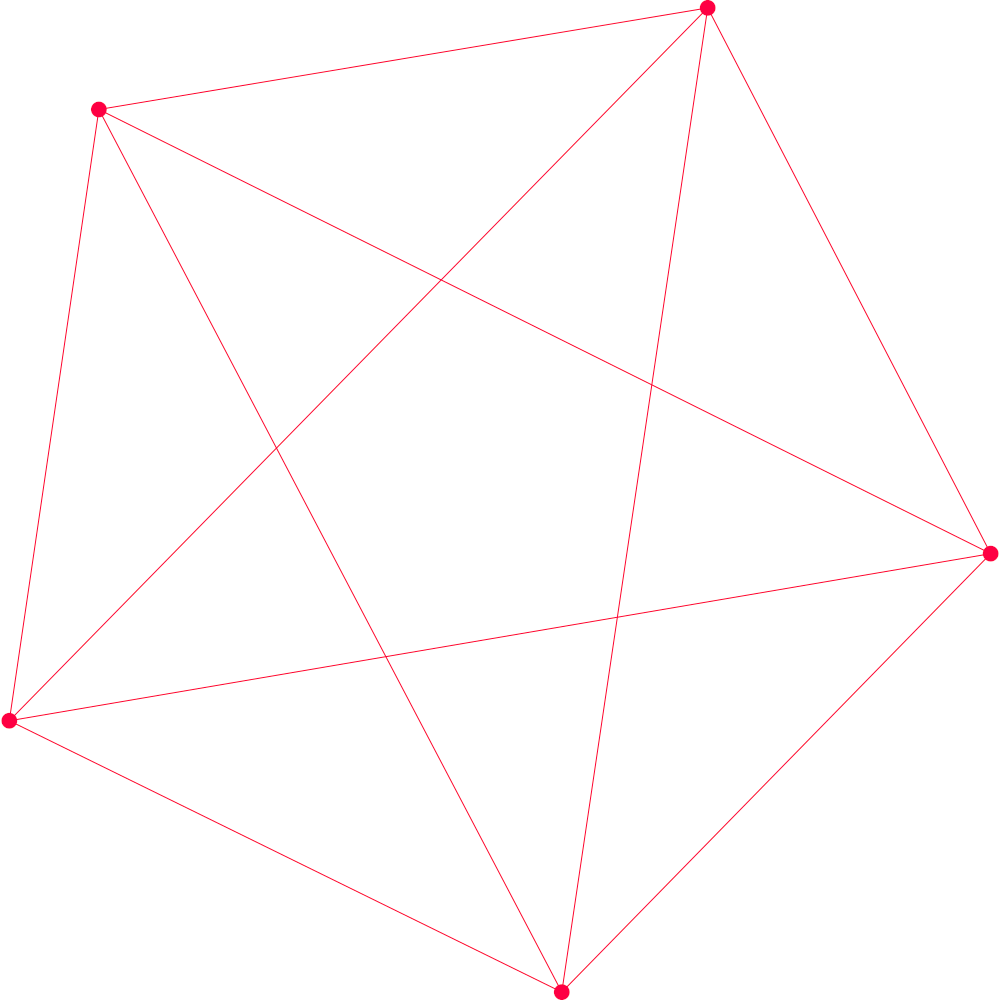
\includegraphics[scale=0.2]{images/complete.png}
    \end{center}
    \caption{SA complete graph. Source Author.}
    \label{fig:complete}
\end{figure}

\section{Illustrative Examples}
\label{examples}

\begin{figure}[!htbp]
    \begin{center}
        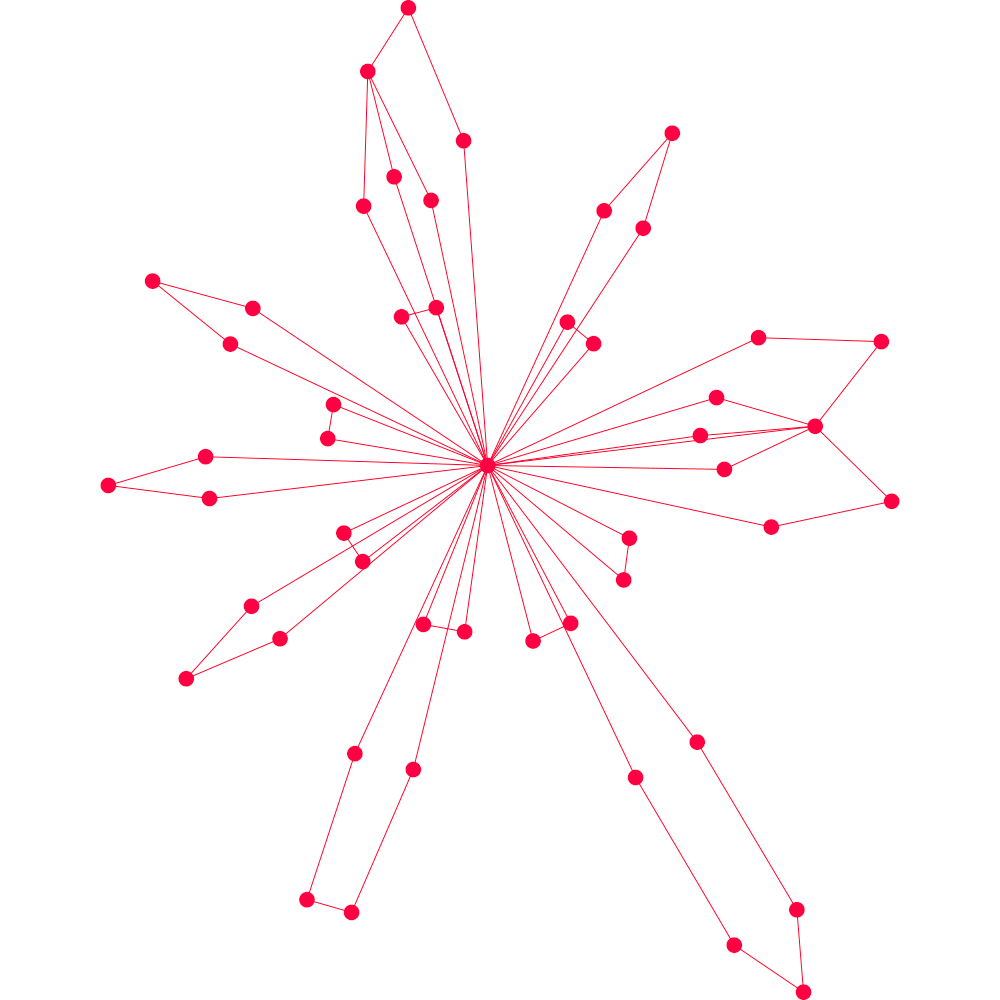
\includegraphics[scale=0.3]{images/scalefree.png}
    \end{center}
    \caption{Scale-free network. Source Author.}
    \label{fig:scalefree}
\end{figure}

\begin{table}[]
\centering
\begin{tabular}{|l|r|r|r|r|}
\hline
\textbf{Property}              & \textbf{CNATool} & \textbf{Gephi} & \textbf{Pajek} & \textbf{SocNetV} \\ \hline
Vertices                       & 50               & 50             & 50             & 50               \\ \hline
Edges                          & 140              & 140            & 140            & 140              \\ \hline
Density                        & 0.05710000       & 0.05700000     & 0.05714286     & 0.05710000       \\ \hline
Average Degree                 & 2.8              & 2.8            & 2.8            & 2.8              \\ \hline
Average Clustering Coefficient & 0.36030000       & 0.34400000     & 0.34431746     & 0.34400000       \\ \hline
Average Shortest Path          & 2.45140          & 2.45100        & 2.45143        & 2.45140          \\ \hline
Diameter                       & 5                & 5              & 5              & 5                \\ \hline
Global Efficiency              & 0.4520           &                &                &                  \\ \hline
\end{tabular}
\caption{Sample scale-free network properties, calculated by the CNATool, Gephi, Pajek and SocNetV programs. Source Author.}
\label{tab:properties}
\end{table}

Optional: you may include one explanatory video that will appear next to your article, in the right hand side panel. (Please upload any video as a single supplementary file with your article. Only one MP4 formatted, with 50MB maximum size, video is possible per article. Recommended video dimensions are 640 x 480 at a maximum of 30 frames/second. Prior to submission please test and validate your .mp4 file at $ http://elsevier-apps.sciverse.com/GadgetVideoPodcastPlayerWeb/verification$. This tool will display your video exactly in the same way as it will appear on ScienceDirect.).

\section{Impact}
\label{impact}

\textbf{This is the main section of the article and the reviewers weight the description here appropriately}

Indicate in what way new research questions can be pursued as a result of the software (if any).

Indicate in what way, and to what extent, the pursuit of existing research questions is improved (if so).

Indicate in what way the software has changed the daily practice of its users (if so).

Indicate how widespread the use of the software is within and outside the intended user group.

Indicate in what way the software is used in commercial settings and/or how it led to the creation of spin-off companies (if so).

\section{Conclusions}
\label{conclusions}

Set out the conclusion of this original software publication.

\section{Conflict of Interest}
We wish to confirm that there are no known conflicts of interest associated with this publication and there has been no significant financial support for this work that could have influenced its outcome.


\section*{Acknowledgements}
\label{acknowledgements}

Funda\c{c}\~{a}o de Amparo \`{a} Pesquisa do Estado da Bahia, 
an agency for induction and promotion of research and scientific and 
technological innovation in the State of Bahia, 
Grant No. 304454/2014-1 MAM. 
The funders had no role in study design, data collection and analysis, 
decision to publish, or preparation of the manuscript.
%% The Appendices part is started with the command \appendix;
%% appendix sections are then done as normal sections
%% \appendix

%% \section{}
%% \label{}

%% References:
%% If you have bibdatabase file and want bibtex to generate the
%% bibitems, please use
%%
%%  \bibliographystyle{elsarticle-num} 
%%  \bibliography{<your bibdatabase>}

%% else use the following coding to input the bibitems directly in the
%% TeX file.

%%\begin{thebibliography}{00}

%% \bibitem{label}
%% Text of bibliographic item

%%\bibitem{}

%%\end{thebibliography}

\section*{References}
\label{references}

\bibliographystyle{elsarticle-num}
\bibliography{references}

\end{document}
\endinput
%%
%% End of file `SoftwareX_article_template.tex'.
